\newif \iftheory 

\theorytrue %\theoryfalse

\newif \ifblind

\blindtrue \blindfalse

\newcommand{\eli}[1]{\textcolor{blue}{[Eli: #1]}}
\newcommand{\meg}[1]{\textcolor{red}{[Megumi: #1]}}
\newcommand{\hannah}[1]{\textcolor{magenta}{[Hannah: #1]}}


% ~~~~~ Modify inside here ~~~~~%
\newcommand{\authorlist}{
% Author 1
Megumi Ando\iftheory\thanks{Computer Science Department, Tufts University, {\tt mando@cs.tufts.edu}}\fi
\and 
% Author 2
Anna Lysyanskaya\iftheory\thanks{Computer Science Department, Brown University, {\tt anna@cs.brown.edu}}\fi
\and 
% Author 3
Hannah Marsh\iftheory\thanks{Computer Science Department, Tufts University, {\tt hmarsh03@cs.tufts.edu}}\fi
\and
% Author 3
Eli Upfal\iftheory\thanks{Computer Science Department, Brown University, {\tt eli@cs.brown.edu}}\fi
}

\newcommand{\institutelist}{}


\newcommand{\titlelist}{\iftheory\begin{bf}\fi
% title
Onion Routing on Sparse Mix-Networks
\iftheory\end{bf}\fi}

% Path to stylefiles
\newcommand{\pathstyles}{./stylefiles}

% Path to preambles
\newcommand{\pathpreambles}{./preambles}

% Path to bibfiles
\newcommand{\pathbibs}{./bibfiles}

% ~~~~~ Modify inside here ~~~~~%


\iftheory
% PLAIN ARTICLE
\documentclass[11pt]{article}

% LNCS (DEFAULT)
\else
%\documentclass[envcountsame, 10pt]{\pathstyles/llncs}
\documentclass[runningheads,a4paper]{llncs}
\ifblind 
\institute{}
\else
\institute{\institutelist}
\fi
\fi

\ifblind 
\author{}
\else
\author{\authorlist} 
\fi
\pagestyle{plain}

\title{\titlelist}

% PREAMBLE
% PREAMBLE
\usepackage[utf8]{inputenc}
\usepackage{amsfonts}
\usepackage{amssymb}
\usepackage{circuitikz}
\usepackage{cite}

\usepackage{xcolor}
\usepackage[
	n,
	operators,
	advantage,
	sets,
	adversary,
	landau,
	probability,
	notions,	
	logic,
	ff,
	mm,
	primitives,
	events,
	complexity,
	asymptotics,
	keys]{cryptocode}
\usepackage{enumitem}
\setlist{nosep}
\usepackage[hidelinks]{hyperref}
%\usepackage{todonotes}

\usepackage{lscape}
\usepackage{mathtools}

% MACROS

% ~~ General

%\DeclareMathOperator*{\argmax}{arg\,max}
%\DeclareMathOperator*{\argmin}{arg\,min}

\renewcommand{\secpar}{\lambda}
\renewcommand{\secparam}{1^\lambda}


% ~~ Formatting
\definecolor{hybrid}{HTML}{0076BA}

\usepackage{caption} 
\captionsetup[table]{skip=10pt}


% ~~~ Begin document ~~~ %
\begin{document}

% ~~~ BODY ~~~ %
\iftheory
\newpage
\thispagestyle{empty}
\tableofcontents
\newpage
\setcounter{page}{1}
\fi

\newcommand{\parties}{\mathsf{Parties}}
\newcommand{\keygen}{\mathsf{KeyGen}}
\newcommand{\formonion}{\mathsf{FormOnion}}
\newcommand{\proconion}{\mathsf{PeelOnion}}
\newcommand{\proconionhelper}{\mathsf{PeelOnionHelper}}
\newcommand{\bruiseonion}{\mathsf{BruiseOnion}}
\newcommand{\polylog}{\mathsf{polylog}}
\newcommand{\early}{\mathsf{early}}
\newcommand{\late}{\mathsf{late}}
\newcommand{\recipient}{\mathsf{Recipient}}
\newcommand{\Bad}{\mathsf{Bad}}

\section{Our Protocol}

Our problem setting consists of $N$ clients (users) and $n$ relays (mixnodes). Assume $N = O(\mathsf{poly}(\lambda))$, and $n = O(\frac{N}{log^2 \lambda})$. While each client has a direct connection to every relay, we model the mixnet of relays as an $r$-regular, $\beta$-expander graph, where $r > 1$. We can write $\beta = \Theta(1/r)$ \cite[Section 2.3]{Hoory2006}.\\

Each client begins with a single message they wish to send privately to another client. We assume that the set of intended recipients is a permutation of the senders, meaning that each client sends and receives exactly one message-bearing onion. Clients are each required to generate $d$ dummy onions (each to be received by the same client) so that the total number of onions in the netowrk is $M = N(d + 1)$. The purpose of the additonal dummy onions to to provide sufficient traffic so that with overwhelming probability with respect to $\lambda$, the difference in volume of onions traversing each edge is negligible. At the start of the protocol, clients must download the current state of the network, which they use to construct a valid routing path of a fixed length $L + 1$ through the mixnet. To bootstrap a path, a client selects the first hop uniformly at random from the set of all relays. The remaining path is then constructed by performing a random walk of length $L$. Finally, the recipient is appended, resulting in a path of length $L + 1$ that traverses randomly through the mixnet and terminates at the intended recipient.\\

The client can then use this path to encrypt their message in successive layers. The innermost layer contains the message encrypted under the recipient’s public key, and each additional layer (added in reverse order of the path) specifies the next hop. Consequently, the innermost layer can only be received and decrypted by the recipient if all preceding layers are properly ``peeled'' by the mixnodes in the selected path.\\

At the beginning of the first round, each client sends their formed onion to the first hop. In subsequent rounds, each relay decrypts the outermost layer and then forwards the peeled onion accordingly.\\

In the final round, the recipient can then reveal the original message (or the empty message if it is a dummy onion).


\subsection{Modeling the Flow of Onions}

Each of the $M$ onions (both message-bearing and dummy) moves through the graph independently according to a simple random walk. Let $P$ represent the $n \times n$ transition matrix of each random walk, where an onion at node $i$ will move to node $j$ with probability:
$$
P_{i,j} = 
\begin{cases}
    \frac{1}{r}, & \text{if there is an edge from $i$ to $j$},\\
    0, & \text{otherwise.}
\end{cases}
$$
Let $\mathbf{p}^{(t)}_{o}$ represent the probability distribution for onion $o \in [M]$ over all nodes at time $t$. Initially, every onion is routed independently and uniformly to a random relay, so define: 
$$
\mathbf{p}^{(1)}_{o,i} = 
\begin{cases}
    1, & \text{if $o$ is routed to node $i$ in the first round,}\\
    0, & \text{otherwise.}
\end{cases}
$$
Thus for every $t > 1$:
$$
\mathbf{p}^{(t+1)}_{o} = P \; \mathbf{p}^{(t)}_{o}
$$
Now define $L^{(t)}_i$ as the number of onions routed to node $i$ in round $t$, and let $e^{(t)}_{i,j}$ represent the number of onions routed from $i$ to $j$ at round $t$.

\subsection{Communication Complexity}

For each message-bearing onion, our protocol requires $\Omega\left(\frac{1}{\lambda^2 \sqrt{\log \lambda}}\right)$ [Thm. \ref{clm:minimum-required-dummy-traffic}] dummy onions to be generated, which provides sufficient traffic so that the fraction of onions sent across any edge in any given round will deviate negligibly from the expectation, $\frac{1}{r}$. This follows from a bound on the server load [Lem. \ref{lem:serverload-bound}] and the edge ratio [Lem. \ref{lem:edgeload-bound}], which are proved below:

\begin{lemma}[Minimum server load] \label{lem:serverload-bound}
    With overwhelming probability, 
    $$
    L^{(t)}_i = \Omega\left( \frac{M}{n} \left(1 - \sqrt{n} \left(1 - \frac{\beta^2}{2}\right)^t\right) \right),
    $$
\end{lemma}
\begin{proof}[Proof of Lemma \ref{lem:serverload-bound}]
Recall:
$$
L^{(t)}_i = \sum_{o \in [M]} \mathbf{p}^{(t)}_{o}.
$$
Applying \cite[Theorem 3.2]{Hoory2006}:
$$
\left| p^{(t)}_i - \frac{1}{n} \right| \leq O\left( \frac{\sqrt{n}}{n} (\eta)^t \right) = O\left( \frac{(\eta)^t}{\sqrt{n}} \right),
$$
where $\eta$ denotes the expansion parameter (second largest eigenvalue of $P$). From Cheeger's inequality, $\eta = 1-\beta^2 / 2$, thus
$$
\left| p^{(t)}_i - \frac{1}{n} \right| \leq O\left( \frac{(1 - \frac{\beta^2}{2})^t}{\sqrt{n}} \right).
$$
By linearity of expectation, 
$$
\left|L^{(t)}_i - \frac{M}{n}\right| \leq O\left( \frac{M \cdot (1 - \frac{\beta^2}{2})^t}{\sqrt{n}} \right),
$$
thus
$$
L^{(t)}_i = \Omega\left( \frac{M}{n} \left(1 - \sqrt{n} \left(1 - \frac{\beta^2}{2}\right)^t\right) \right),
$$

\end{proof}

Next we bound the fraction of onions $i$ sends across an edge:

\begin{lemma}[Maximum edge ratio] \label{lem:edgeload-bound}
    With overwhelming probability, 
    $$
     \frac{e^{(t)}_{i,j}}{L^{(t)}_i} = \frac{1}{r} + O\left(\sqrt{\frac{n(\log \lambda \cdot \omega(1) + \log r)}{Mr \left(1 - \sqrt{n} \left(1 - \frac{1}{2r^2}\right)^t\right)}}\right)
    $$
\end{lemma}
\begin{proof}[Proof of Lemma \ref{lem:edgeload-bound}]

Define $e^{(t)}_{i,j}$ as the number of onions routed from $i$ to $j$ at round $t$. Then $\mathbb{E}[e^{(t)}_{i,j}] = \frac{L^{(t)}_i}{r}$. By Lemma \ref{lem:chernoff-deviation}, we bound with overwhelming probability in $\lambda$:
$$ 
e^{(t)}_{i,j} \leq \frac{L^{(t)}_i}{r} + \sqrt{\frac{3L^{(t)}_i}{r}(\log \lambda \cdot \omega(1) + \ln r)})
$$
Thus
$$ 
\frac{e^{(t)}_{i,j}}{L^{(t)}_i} \leq \frac{1}{r} + \sqrt{\frac{3(\log \lambda \cdot \omega(1) + \ln r)}{r \cdot L^{(t)}_i}}
$$
Substituting $L^{(t)}_i = \Omega\left( \frac{M}{n} \left(1 - \sqrt{n} \left(1 - \frac{\beta^2}{2}\right)^t\right) \right)$,
\begin{align*}
    \frac{e^{(t)}_{i,j}}{L^{(t)}_i} &\leq \frac{1}{r} + \sqrt{\frac{3(\log \lambda \cdot \omega(1) + \ln r)}{\Omega\left( \frac{Mr}{n} \left(1 - \sqrt{n} \left(1 - \frac{\beta^2}{2}\right)^t\right) \right)}}\\
    &= \frac{1}{r} + O\left(\sqrt{\frac{n(\log \lambda \cdot \omega(1) + \log r)}{Mr \left(1 - \sqrt{n} \left(1 - \frac{1}{2r^2}\right)^t\right)}}\right)\\
\end{align*}
\end{proof}


We now prove the main result of this section:

\begin{theorem}[Minimum required dummy traffic] \label{clm:minimum-required-dummy-traffic}
    If for each message-bearing onion, $\Omega\left(\frac{1}{\lambda^2 \sqrt{\log \lambda}}\right)$ dummy onions are generated, then the number of onions traversing any edge before round $t$ will deviate negligibly from the expectation.
\end{theorem}
\begin{proof}[Proof of Lemma \ref{clm:minimum-required-dummy-traffic}]
Requiring:
\begin{align*}
    \frac{e^{(t)}_{i,j}}{L^{(t)}_i} &= \frac{1}{r} + O\left(\sqrt{\frac{n(\log \lambda \cdot \omega(1) + \log r)}{Mr \left(1 - \sqrt{n} \left(1 - \frac{1}{2r^2}\right)^t\right)}}\right) &= \mathsf{negl}(\lambda)\\
    &\Rightarrow \frac{1}{r} + O\left(\sqrt{\frac{n(\log \lambda \cdot \omega(1) + \log r)}{Mr \left(1 - \sqrt{n} \left(1 - \frac{1}{2r^2}\right)^t\right)}}\right) &= \lambda + \exp(- \omega(1))
\end{align*}
Solving for $M$:
\begin{align*}
    \frac{n(\log \lambda \cdot \omega(1) + \log r)}{Mr \left(1 - \sqrt{n} \left(1 - \frac{1}{2r^2}\right)^t\right)} &\geq \frac{1}{C}\left(\lambda + \exp(- \omega(1)) - \frac{1}{r}\right)^2\\
    M &= \Omega\left(\frac{n(\log \lambda \cdot \omega(1) + \log r)}{r \left(1 - \sqrt{n} \left(1 - \frac{1}{2r^2}\right)^t\right)\left(\lambda + \exp(- \omega(1)) - \frac{1}{r}\right)^2}\right)\\
\end{align*}
Thus each client must generate at least $d_\text{min}$ dummy onions, where
\begin{align*}
    d_\text{min} &= \Theta\left(\frac{n(\log \lambda \cdot \omega(1) + \log r)}{Nr \left(1 - \sqrt{n} \left(1 - \frac{1}{2r^2}\right)^t\right)\left(\lambda + \exp(- \omega(1)) - \frac{1}{r}\right)^2}\right)\\
                 &= O\left(\frac{1}{\lambda^2 \sqrt{\log \lambda}}\right)\\
                    % &= \Theta\left(\frac{\omega(1)}{\log\lambda \left(1 - \sqrt{n} \left(1 - \frac{1}{2r^2}\right)^t\right)\left(\lambda + \exp(- \omega(1))\right)^2}\right)\\
                    % &= \Theta\left(\frac{\omega(1)}{\left(1 - \sqrt{n} \left(1 - \frac{1}{2r^2}\right)^t\right)\left(\lambda^2 \log \lambda + \lambda \log \lambda \exp(- \omega(1))\right)}\right)\\
                    % &= \Theta\left(\frac{\omega(1)}{\left(1 - \sqrt{n} \exp(-t) \right)\left(\lambda^2 \log \lambda + \lambda \log \lambda \exp(- \omega(1))\right)}\right)\\
                    % &= \Theta\left(\frac{\omega(1)}{\left(1 - \frac{\sqrt{N}}{\log \lambda \exp(t)} \right)\left(\lambda^2 \log \lambda + \lambda \log \lambda \exp(- \omega(1))\right)}\right)\\
                    % &= \Theta\left(\frac{\omega(1)}{(\lambda^2 \log \lambda + \lambda \log \lambda \exp(- \omega(1))) - \frac{\sqrt{N}(\lambda^2 \log \lambda + \lambda \log \lambda \exp(- \omega(1)))}{\log \lambda \exp(t)}}\right)\\
                    % &= \Theta\left(\frac{\omega(1)}{\frac{\log \lambda \exp(t)(\lambda^2 \log \lambda + \lambda \log \lambda \exp(- \omega(1))) - \sqrt{N}(\lambda^2 \log \lambda + \lambda \log \lambda \exp(- \omega(1)))}{\log \lambda \exp(t)}}\right)\\
                    % &= \Theta\left(\frac{\omega(1)\log \lambda \exp(t)}{\log \lambda \exp(t)(\lambda^2 \log \lambda + \lambda \log \lambda \exp(- \omega(1))) - \sqrt{N}(\lambda^2 \log \lambda + \lambda \log \lambda \exp(- \omega(1)))}\right)\\
                    % &= \Theta\left(\frac{\omega(1)\log \lambda \exp(t)}{\log \lambda \exp(t) \lambda^2 \log \lambda + \log \lambda \exp(t) \lambda \log \lambda \exp(- \omega(1)) - \sqrt{N} \lambda^2 \log \lambda - \sqrt{N} \lambda \log \lambda \exp(- \omega(1))}\right)\\
                    % &= \Theta\left(\frac{\omega(1) \exp(t)}{\lambda^2 \log \lambda \exp(t) + \lambda \log \lambda \exp(t - \omega(1)) - \sqrt{N} \lambda^2 - \sqrt{N} \lambda \exp(- \omega(1))}\right)\\
                    % &= \Theta\left(\frac{\omega(1) \exp(t) / \lambda}{\lambda \log \lambda \exp(t) + \log \lambda \exp(t - \omega(1)) - \sqrt{N} \lambda - \sqrt{N} \exp(- \omega(1))}\right)\\
                    % &\leq \Theta\left(\frac{1}{\lambda (\log \lambda - \frac{\sqrt{N}}{\exp(t)})}\right)\\
\end{align*}
% For $t = \Omega(\log \lambda)$.
% \begin{align*}
%     d_\text{min} &= O\left(\frac{1}{\lambda \log \lambda}\right)
% \end{align*}
\end{proof}


\subsection{Network Adversary}

\begin{theorem} \label{clm:network}
    $\Pi_x$ is statistically private from the network adversary when $d = \Omega\left(\frac{1}{\lambda^2 \sqrt{\log \lambda}}\right)$ and $L = \Omega(\log \lambda)$, where $\lambda \in \mathbb{N}$ denotes the security parameter.\\
\end{theorem}


\begin{proof} [Proof of Theorem~\ref{clm:network}]
At the start of the protocol, the adversary knows the exact location of every sender's onion. Let $O$ represent one of these onions, and let $S \in [n]$ be its initial location. For each round $t \in [1 \dots L]$, we represent the adversary’s belief about the location of $O$ as a probability distribution vector $\mathbf{h}^{(t)} = (\mathbf{h}^{(t)}_1, \mathbf{h}^{(t)}_2, \dots, \mathbf{h}^{(t)}_n)$ over the set of nodes $i \in [n]$. Specifically, $\mathbf{h}^{(t)}_i$ denotes the adversary's best guess of the probability that $O$ is at node $i$ during round $t$. Initially, we define

$$
\mathbf{h}^{(1)}_i =
\begin{cases}
    1, & \text{if } i = S,\\
    0, & \text{otherwise.}
\end{cases}
$$

After every round, the adversary updates their belief based on the observed volumes of onions traversing each edge. Thus we model the belief vector as the probability distribution of a time-inhomogeneous random walk starting from $S$, and updating according to the fractions of each nodes onions emitted on its edges every round.\\

The adversary's belief of $O$'s location evolves according to the transition matrix $H$, where:
$$
H^{(t)}_{i,j} = 
\begin{cases}
    \frac{e^{(t + 1)}_{i,j}}{L^{(t + 1)}_i}, & \text{if $L^{(t + 1)}_i > 0$},\\
    0, & \text{otherwise.}
\end{cases}
$$

Here:
$$
\frac{e^{(t + 1)}_{i,j}}{L^{(t + 1)}_i} = \frac{\text{number of onions $i$ sends to $j$ in round $t + 1$}}{\text{total number of onions $i$ sends in round $t + 1$}},
$$

From Theorem \ref{clm:minimum-required-dummy-traffic}, we showed that every $\frac{e^{(t + 1)}_{i,j}}{L^{(t + 1)}_i}$ will be negligibly different from $\frac{1}{r}$. Thus:
$$
H^{(t)}_{i,j} \approx_s P = 
\begin{cases}
    \frac{1}{r}, & \text{if $i$ and $j$ are neighbors},\\
    0, & \text{otherwise.}
\end{cases}
$$

Therefore, $\mathbf{h}^{(t)} \approx_s \mathbf{p}^{(t)}_O$, meaning the adversary's belief vector of where $O$ is at any given round is indistinguishable from the probability vector of $O$'s simple random walk (originating at $S$ in round 1). That is to say that for an onion observed being routed to a node $i$ in round $t$, the adversary's best guesss of which of $i$'s neighbors the onion will be routed to in round $t + 1$ is negligibly greater than a purely random guess ($\frac{1}{r}$).\\\\
Thus the minimum number of steps required to guarantee every $H^{(t)}_{i,j} \approx_s \mathbf{\frac{1}{n}}$ is the mixing time of a simple random walk originating at $S$:
\begin{align*}
    t_\text{mix}(\epsilon = \mathsf{negl}(\lambda)) &= O\left(\frac{\log(\mathsf{poly}(\lambda))}{\beta^2}\right)\\
    &= O\left(\frac{\log \lambda}{\Theta(1/r^2)}\right)\\
    &= O\left(\log \lambda\right).
\end{align*}

Therefore, by the end of the protocol (after $L = \Omega(\log \lambda)$ rounds), the adversary's believe about $O$'s location is indistinguishable from uniform. Thus $\Pi_x$ achieves statistical privacy against the network adversary.

\end{proof}

\clearpage

\subsection{Passive Adversary}

\begin{theorem} \label{clm:passive}
    $\Pi_x$ is statistically private against a passive adversary who can monitor up to a constant fraction $\chi < \frac{1}{2}$ of the servers. Assume $d = \Omega\left(\frac{1}{\lambda^2 \sqrt{\log \lambda}}\right)$ and $L = \Omega(\log^k \lambda)$ for $k > 1$, where $\lambda \in \mathbb{N}$ denotes the security parameter.\\
\end{theorem}

\begin{proof} [Proof of Theorem~\ref{clm:passive}]

Let $C$ denote the set of monitored nodes, where $|C| = \chi < \frac{n}{2}$. Similar to the network adversary setup, at the start of the protocol, the adversary knows the exact location of every sender's onion. Let $O$ represent one of these onions, and let $S \in [n]$ be its initial location. We will show that with overwhelming probability in $\lambda$, $O$ has at least $\Omega(\log \lambda)$ honest parties in its routing path. 

% Lemma: Simple ranodm walker starts in some subset < 1/2 n nodes. Then by mixing lemma, with overwhelming probability the walker will leave the subset after $O(\log \lambda)$ time steps. Now, suppose an onion’s path is of total length 
% $$
% L = \Omega(\log^2 \lambda).
% $$ 
% We can partition this path into 
% $$
% K = \Omega\Bigl(\frac{L}{\log \lambda}\Bigr) = \Omega(\log \lambda)
% $$ 
% consecutive subpaths (or blocks), each of length $O(\log \lambda)$. By the argument above, in each such block the probability that every hop is adversarial is negligible. Therefore, by a union bound over these $K$ blocks), with overwhelming probability at least one hop in each block must be honest.

% Thus, the entire path of length $\Omega(\log^2 \lambda)$ will contain at least 
% $$
% \Omega(\log \lambda)
% $$ 
% honest hops.

% Let $\mathbf{p}^{(t)}$ denote the probability distribution of the onion's location after $t$ honest hops. In the network adversary case (where every hop contributes to mixing) it has been shown that after
% $$
% t_{\text{mix}} = \Omega(\log \lambda)
% $$
% steps the distribution is statistically close to the uniform distribution; that is, for an onion $O$ with initial location $S$,
% $$
% \Bigl\|\mathbf{p}_O^{(t_{\text{mix}})} - \frac{1}{n}\mathbf{1}\Bigr\|_{\text{TV}} \leq \text{negl}(\lambda),
% $$
% where $\|\cdot\|_{\text{TV}}$ is the total variation distance.

% Since, conditioned on the event $\mathcal{E}$, an onion experiences at least $c\log \lambda \ge t_{\text{mix}}$ honest hops, its probability distribution is mixed to within negligible statistical distance from uniform. Note that adversarial hops, while not contributing to mixing, do not adversely affect this argument because the overall state is updated only upon an honest hop.

% Let $\mathbf{h}^{(L)}$ be the adversary's belief (which may incorporate the non-mixing adversarial hops) about the onion's location after $L$ rounds. We have
% $$
% \Bigl\|\mathbf{h}^{(L)} - \frac{1}{n}\mathbf{1}\Bigr\|_{\text{TV}} \leq \Pr[\overline{\mathcal{E}}] + \Pr[\mathcal{E}]\cdot \text{negl}(\lambda).
% $$
% This probability is negligible in $\lambda$, it follows that
% $$
% \Bigl\|\mathbf{h}^{(L)} - \frac{1}{n}\mathbf{1}\Bigr\|_{\text{TV}} \leq \text{negl}(\lambda).
% $$
% Thus, after $L = \Omega(\log^2 \lambda)$ rounds, the adversary's belief about the location of any onion is statistically indistinguishable from the uniform distribution.



% Let $C$ denote the set of monitored nodes, where $|C| = \chi < \frac{n}{2}$. Similar to the network adversary setup, at the start of the protocol, the adversary knows the exact location of every sender's onion. Let $O$ represent one of these onions, and let $S \in [n]$ be its initial location.\\\\
% To model the adversary's belief as a Markov chain, we construct a transformed, weighted, directed graph $G'=(V',E')$ as follows:\\

% \begin{enumerate}
%     \item Initially, $G'$ is a copy of $G$. Replace each undirected edge with two directed edges in opposite directions. Assign each edge a weight of $\frac{1}{r}$. Let $W(i,j)$ denote the weight of the edge from $i$ to $j$.
%     \item For each $c \in C$, let $\mathcal{N}(c)$ denote its set of neighbors in $G'$. 
%     \begin{enumerate}
%         \item For every ordered pair of neighbors $(u, v) \in \mathcal{N}(c) \times \mathcal{N}(c)$:
%         \begin{enumerate}
%             \item Introduce a new vertex labeled `$ucv$' in $G'$.
%             \item Add directed edge $(u, ucv)$. Assign a weight of $W(u, ucv) = W(u,c) / r$.
%             \item Add a directed edge $(ucv, v)$. Assign a weight of $W(ucv, v) = 1$.
%         \end{enumerate}
%         \item Remove $c$ (along with its incident edges) from $G'$.
%     \end{enumerate}
% \end{enumerate}

% \begin{center}
%     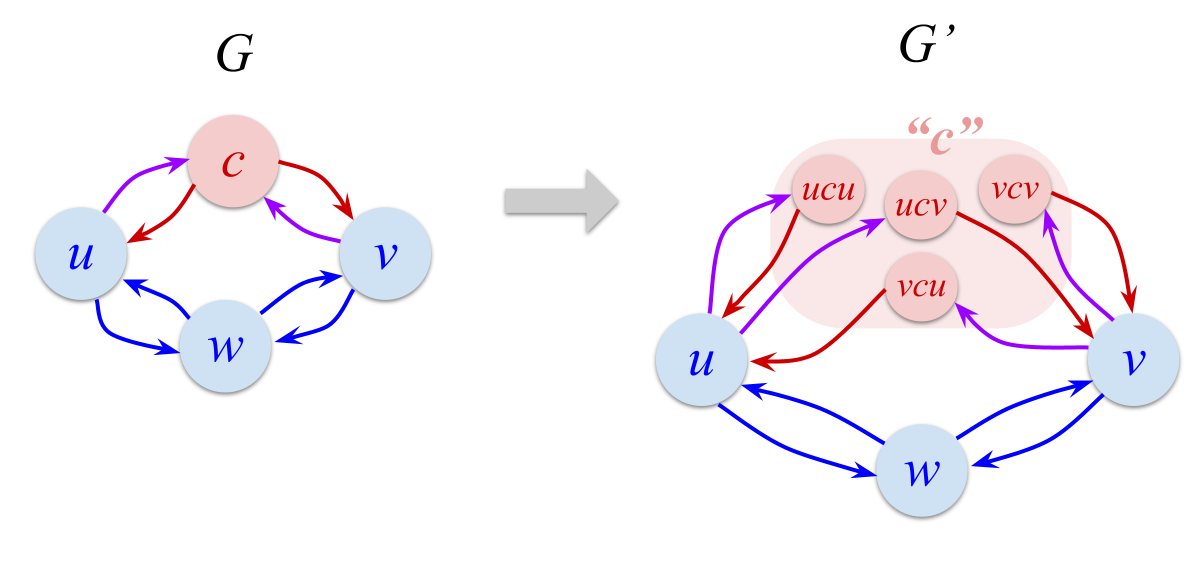
\includegraphics[width=250pt]{template/figures/transformation_of_G (1).png}
% \end{center}
% Thus the path $u \to c \to v$ of a onion in $G$ is “observed” by the adversary as the two-step route:
% $$
% u \to (ucv) \to v,
% $$
% in $G'$, where $ucv$ has exactly one incoming edge (from $u$) and one outgoing edge (to $v$). In this way, the ``probability of being $O$'' for an onion leaving $u$ (to $c$) will not change by the time it enters $v$ (from $c$). This models the lack of mixing happening at corrupted nodes, and thus the adversary’s view evolves as a simple random walk on our transformed graph $G'$, governed by the transition matrix $H$, where  
% $$
% H_{i,j} =
% \begin{cases}
% 1, & \text{if } i \text{ is a new vertex } (ucv \in C') \text{ and } j = v,\$$1mm]
% \frac{1}{r}, & \text{if } i \text{ is an honest party and } (i,j)\in E',\$$1mm]
% 0, & \text{otherwise.}
% \end{cases}
% $$
% For example, below is the Markov chain of a random walk on $G$ and on its transformation $G'$ (red nodes represent corrupted parties):
% \begin{center}
%     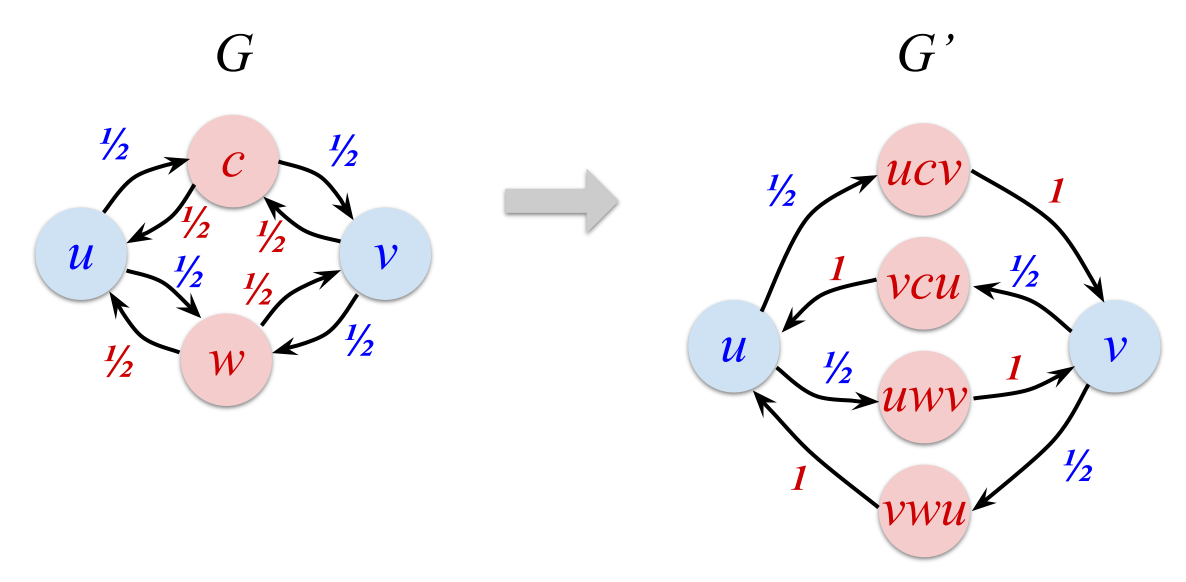
\includegraphics[width=250pt]{template/figures/transformation_of_G_markkov_chain.png}
% \end{center}

% Our goal is to show that the expansion properties of $H$ (i.e., $1 - \lambda_2(H)$) is not significantly degraded by this transformation. The important things that are preserved in $G'$ is the number of directed edges\\

% Any cut in $G'$ that isolates many shortcut vertices (corrupted nodes) must also separate a significant number of their associated honest neighbors (preserving overall connectivity). Formally, let $R = V \setminus C$ denote the subset of honest relays. Then its edge boundary satisfies:
% $$
% \frac{\text{edges}(R, V' \setminus S)}{\text{vol}(S)} \geq \Omega(\beta),
% $$
% which implies:
% $$
% 1 - \lambda_2(H) \geq \Omega(\beta^2).
% $$

% For any initial distribution, the time required to reach a distribution within $\epsilon = \mathsf{negl}(\lambda)$ (of uniform is given by:  
% $$
% t_{\mathrm{mix}}(\epsilon) = O\biggl(\frac{\log |V'|}{\beta^2}\biggr).
% $$
% Since $|V'| = O(n)$ and $n = O(\mathsf{poly}(\lambda))$, we have  
% $$
% \log |V'| = O(\log \lambda).
% $$
% Thus, for sufficiently large $\lambda$, the adversary's belief distribution mixes within  
% $$
% t_{\mathrm{mix}}(\epsilon = \mathsf{negl}(\lambda)) = O(\log \lambda).
% $$
% This means that after $L = \Omega(\log \lambda)$ rounds, the adversary’s belief distribution over $V'$ becomes statistically close to uniform.

    
\end{proof}

\begin{lemma}\label{lem:escape-time}
Let $C \subset [n]$ be any subset of relays with $|C| < \frac{n}{2}$. Then with overwhelming probability in $\lambda$, a random walk of length $\Omega(\log^c \lambda)$ for $c > 1$ will visit $\Omega(\log^c \lambda)$ relays $\not\in C$ with overwhelming probability in $\lambda$.
\end{lemma}
\begin{proof}[Proof for Lemma \ref{lem:escape-time}]
Let $t_n$ be the number of visits to $C$ in $t$ steps, where $\mathbb{E}[t_n] = \frac{|C|t}{n}$. Then \cite[Theorem 2.1]{gillman1998chernoff} states that for any deviation $\gamma > 0$:
$$
\Pr[t_n - \frac{t|C|}{n} \geq \gamma] \leq (1 + \gamma \epsilon / 10t) N_q e^{-\gamma^2 \epsilon / 20t}.
$$
where $N_q = 1$ accounts for the starting distribution, and $\epsilon = 1 - \lambda_2$ is the spectral gap of the expander. Then we can write:
\begin{align*}
    \Pr[t_n - \frac{t|C|}{n} \geq \gamma] \leq (1 + \frac{\gamma \cdot \Theta\left(\frac{1}{r}\right)}{10t}) \exp(-\frac{\gamma^2 \cdot \Theta\left(\frac{1}{r}\right)}{20t})
\end{align*}
Requiring $\Pr[t_n - \frac{t|C|}{n} \geq \gamma] = \mathsf{negl}(\lambda)$,
\begin{align*}
    \frac{\gamma^2 \cdot \Theta\left(\frac{1}{r}\right)}{20t} &= \log^\delta \lambda &\text{for any $\delta > 1$}\\
    \Rightarrow \gamma &= \sqrt{t \cdot \log^\delta \lambda}
\end{align*}
Thus with overwhelming probability in $\lambda$, 
\begin{align*}
    t_n &< \frac{t|C|}{n} + \sqrt{t \cdot \log^\delta \lambda}\\
    &< \frac{t}{2} + \sqrt{t \cdot \log^\delta \lambda}\\
    t - t_n &\geq \frac{t}{2} - \sqrt{t \cdot \log^\delta \lambda}\\
\end{align*}
This gives a bound for the number of visits $\not\in C$. Specifically when $t = \Omega(\log^c \lambda)$ for $c > 1$
\begin{align*}
    t - t_n &= \Omega(\log^c \lambda - \log^{\frac{c + \delta}{2}}\lambda)\\
    &= \Omega((\log^c \lambda)(1 - \log^{\frac{\delta - c}{2}}\lambda))\\
\end{align*}
Since $c > 1$, a valid choice of $\delta$ is $\delta = \frac{c + 1}{2}$, which implies:
$$
\frac{\delta - c}{2} < 0.
$$
Therefore:
\begin{align*}
    t - t_n &= \Omega(\log^c \lambda) \cdot \Theta(1 - \log^{\frac{\delta - c}{2}}\lambda)\\
    &= \Omega(\log^c \lambda) \cdot \Theta(1)\\
\end{align*}
We conclude that after $t = \Omega(\log^c \lambda)$ steps, a random walk will visit $\Omega(\log^c \lambda)$ vertices $\not\in C$ with overwhelming probability in $\lambda$.
\end{proof}



\clearpage
% ~~~ REFERENCES ~~~ %
%\bibliographystyle{plain}
%\bibliographystyle{is-alpha}
\bibliographystyle{stylefiles/alpha-short}
\bibliography{template/bibfiles/abbrev3,template/bibfiles/crypto,template/bibfiles/anon,template/bibfiles/refs} 

\appendix 

\clearpage

% MORE PROOFS
\section{Supplementary proofs} \label{sec:proofs}


\begin{lemma} \label{lem:chernoff-deviation} Consider a random experiment with $n$ equally likely outcomes conducted over $N$ independent Poisson trials. Let $\lambda$ denote any sufficiently large natural number. Let $X_i$ denote the number of times an outcome $i$ occurred after $N$ trials. Then with overwhelming probability w.r.t. $\lambda$, every outcome $i \in [n]$ will deviate from $\mathbb{E}[X_i] = \frac{N}{n}$ no more than:
$$ 
\sqrt{\frac{3N}{n}(\Theta((\log \lambda) \cdot \alpha(\lambda)) + \ln n)}).
$$
\end{lemma} 

\begin{proof}[Proof of Lemma~\ref{lem:chernoff-deviation}]

Let $X_i$ denote the number of times some outcome $i \in [n]$ occurred after $N$ trials. Then $\mathbb{E}[X_i]$ = $\frac{N}{n}$, and it follows from Chernoff bounds~\cite[Cor.~4.6]{MU05} that for all $0 < \delta < 1$:
$$
\Pr\left(|X_i - \frac{N}{n}| \geq \delta \cdot \frac{N}{n} \right) \leq 2 e^{-\frac{\delta^2 \cdot N}{3n}}.
$$
Applying the union bound over all $n$ outcomes, we get:
$$
\Pr\left(\exists i \in [n]: |X_i - \frac{N}{n}| \geq \delta \cdot \frac{N}{n} \right) \leq n \cdot 2 e^{-\frac{\delta^2 \cdot N}{3n}} = 2 e^{\ln n -\frac{\delta^2 \cdot N}{3n}}.
$$

Next, we want to solve for $\delta$, requiring a negligible probability:

\begin{align*}
2 e^{\ln n -\frac{\delta^2 \cdot N}{3n}} &= \mathsf{negl}(\lambda)\\
\frac{\delta^2 \cdot N}{3n} - \ln n &= \omega(\log \lambda)\\
\delta &= \sqrt{\frac{3n}{N}(\omega(\log \lambda) + \ln n)}\\
\end{align*}

However, $\omega(\log \lambda)$ can be any function of \(\lambda\) that grows strictly faster than logarithmic and can be written as $\log \lambda \cdot \omega(1)$. Thus
$$
\delta = \sqrt{\frac{3n}{N} (\omega(1) \cdot \log \lambda + \log n)}
$$

Thus, with overwhelming probability (w.r.t. $\lambda$), we have:
$$
X_i \leq \frac{N}{n} + \sqrt{\frac{3N}{n}(\Theta((\log \lambda) \cdot \alpha(\lambda)) + \ln n)})
$$

\end{proof}

\end{document}